\section{Introduction}\label{sec:intro}

The distributivity of information and services over the Internet has changed all aspects
of life, and science is not an exception. We anticipate that the systems currently
investigated in the community will eventually change scientific practice and that they
will have a strong societal impact, provided that they can inter-operate to cover the
whole work-flow of scientific research, education and application. 
\begin{wrapfigure}{r}{6.5cm}\vspace{-.6cm}
  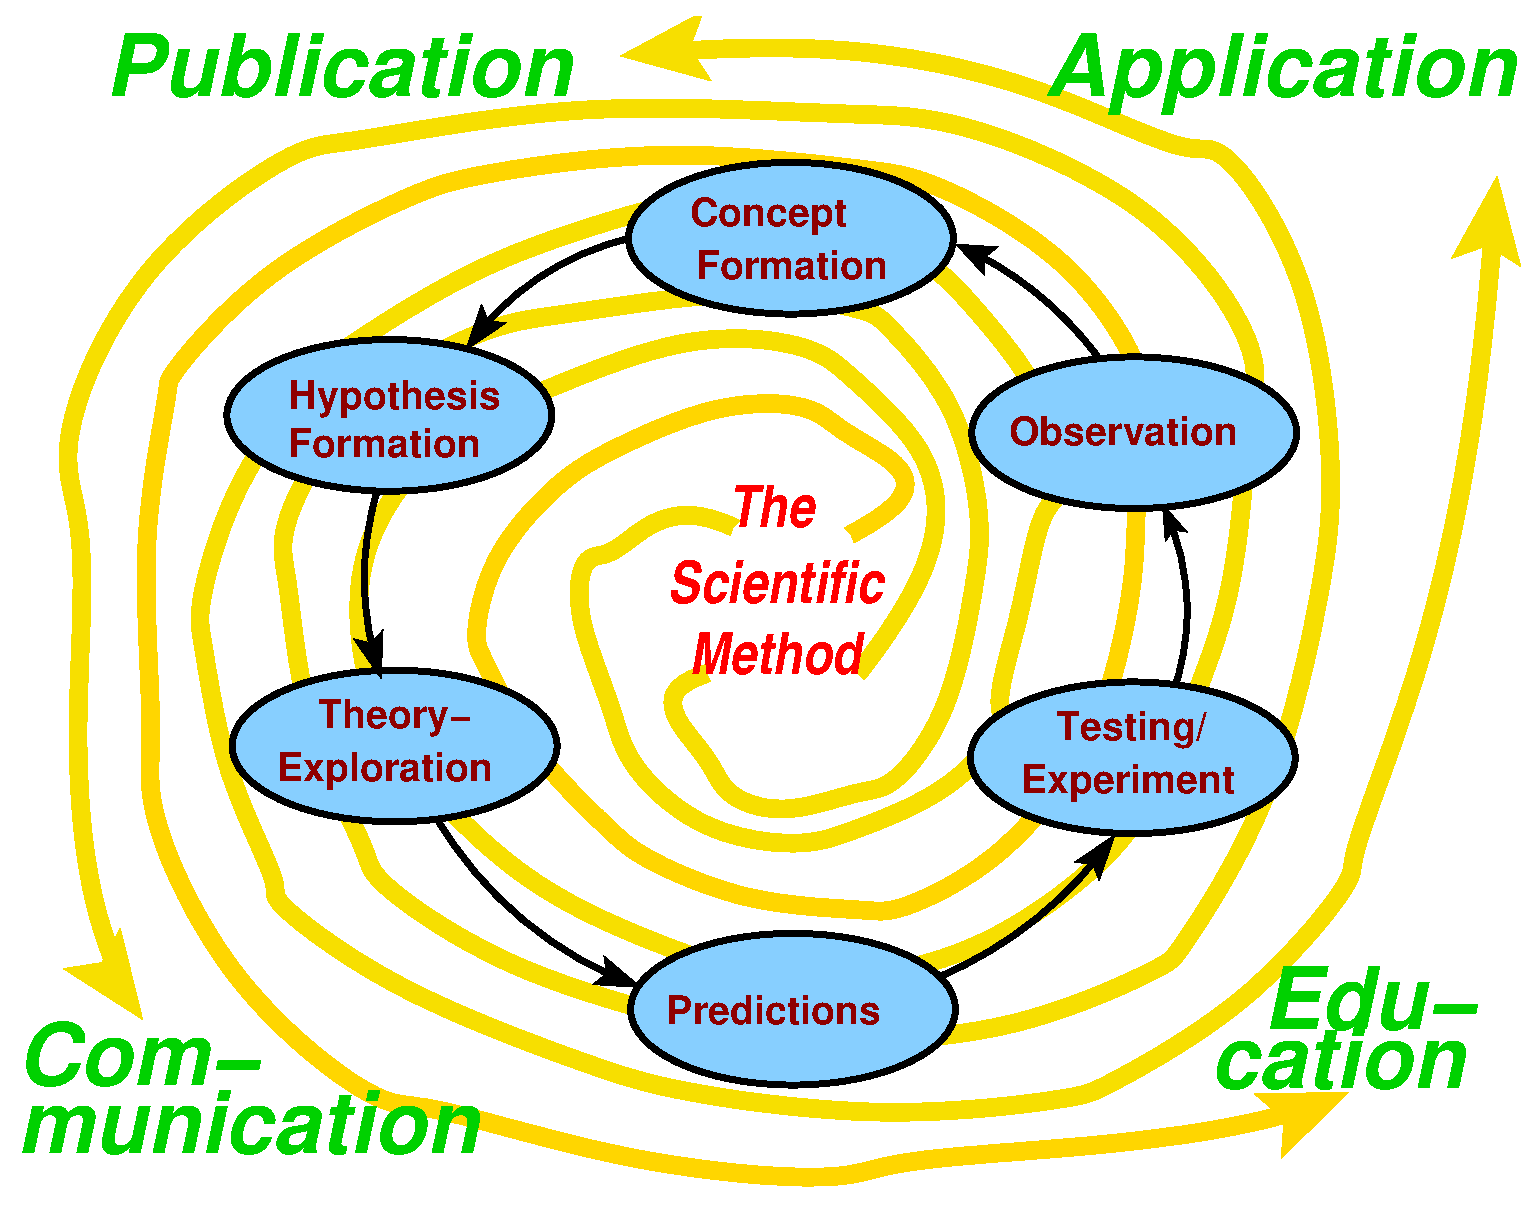
\includegraphics[width=6.5cm]{sci-method}\vspace{-.3cm}
  \caption{The Scientific Method}\label{fig:nw-Methode}\vspace{-.6cm}
\end{wrapfigure}
To further this vision we need to develop, implement, and provide semantic-based and
context-aware techniques for acquiring, organizing, processing, sharing and using
knowledge in science.
 
Our starting point is the view of the {\emph{scientific method}} as a spiral (see
Fig.~\ref{fig:nw-Methode}), where we have our focus on physics here.  In this view,
scientific research in physics moves in a spiral trajectory from original ideas to results
and even applications. Ideas pass through the processes of observation of natural
processes, then of concept formulation to describe these. These allow scientists to
express initial theories about (quantitative laws of nature governing) them, which are
then explored (what are the consequences of the model assumptions) leading to predictions
about processes that can be verified or falsified (to a certain degree) experimentally.
These experiments usually lead to new observations, starting the next round in the spiral
until a quantitative (mathematically formulated) \textit{theory} predicting exclusively
correct results from experiments is formulated.  Observables in physics have to be
suitably found such that they can be physically measured, their algebraic counterparts
being then candidates for building stones of a theory.  The semantics of mathematics as
such is more confined, searching for logically correct sets of rules.

At the moment, most of the steps in Fig.~\ref{fig:nw-Methode} are separately supported by
software systems, e.g.  literature searches in {\googlescholar} or {\wikipedia}, theory
exploration in computer algebra systems like {\mathematica}, and experiments in simulation
systems. But the systems are, by and large, not able to inter-operate since they use
differing data formats, make differing model assumptions, and are bound to an implicitly
given context that is only documented in publications about the systems. For instance,
copy-and-paste from {\googlescholar} or {\wikipedia} to {\mathematica} or a simulation
system is impossible because of this format problem. Moreover, where possible, copy and
paste can be very dangerous, since computer algebra systems make differing assumptions on
the Computercode-libraries, 
the simulation systems are based on\footnote{A simple example, where the lack of
explicit context led to a very expensive failure was the September 1999 loss of a \$125
million Mars orbiter, which crashed on Mars. The cause was that NASA used for its
specifications metric units, but the Lockheed Martin engineers misinterpreted the data
assuming they were given using Imperial units of measurement.}.

We are set here to arrive at a content markup format for physics. Early concept
discussions and visions~\cite{Hilf:texdocc,PML:web,Hilf:guestrow,Hilf:p05} have not led to
a realization in terms of an encoding, since the problem was attacked from the ground up.
In this paper we will build the bridge from vision to a usable markup language by
extending the {\omdoc} ({\underline{O}pen} {\underline{M}athematical}
{\underline{Doc}uments}) format~\cite{Kohlhase:omdoc1.2} by an infrastructure for
(physical) systems, observables and experiments and call this new module and the extended
system {\physml} (Physics Markup Language). Since we can now share all the infrastructure
--- in particular the theory and statement levels --- with mathematics, the language
design for {\physml} becomes feasible.


%%% Local Variables: 
%%% mode: stex
%%% TeX-master: "mkm06"
%%% End: 

% LocalWords:  cience ech logy ngineering athematical uments ciences echnology
% LocalWords:  athematics stex mkm
